\documentclass[12pt]{article}
\usepackage{fullpage} 
\usepackage{microtype}      % microtypography
\usepackage{array}
\usepackage{amsmath,amssymb,amsfonts}
\usepackage{amsthm}
\usepackage{graphicx}

%% Header
\usepackage{fancyhdr}
\fancyhf{}
\fancyhead[C]{CS 136 - 2022s - Checkpoint1 Submission}
\fancyfoot[C]{\thepage} % page number
\renewcommand\headrulewidth{0pt}
\pagestyle{fancy}

\usepackage[headsep=0.5cm,headheight=2cm]{geometry}

%% Hyperlinks always blue, no weird boxes
\usepackage[hyphens]{url}
\usepackage[colorlinks=true,allcolors=black,pdfborder={0 0 0}]{hyperref}

%%% Doc layout
\usepackage{parskip}
\usepackage{times}

%%% Write out problem statements in blue, solutions in black
\usepackage{color}
\newcommand{\officialdirections}[1]{{\color{blue} #1}}

%%% Avoid automatic section numbers (we'll provide our own)
\setcounter{secnumdepth}{0}

\begin{document}
~~\\ %% add vert space

{\Large{\bf Student Names: Alex Lobo and Nate Davis}}


{\Large{\bf Collaboration Statement:}}

Turning in this assignment indicates you have abided by the course Collaboration Policy:

\url{www.cs.tufts.edu/comp/136/2022s/index.html#collaboration-policy}

Total hours spent: TODO

We consulted the following resources:
\begin{itemize}
\item TODO
\item TODO
\item $\ldots$	
\end{itemize}

These are the official instructions for checkpoint 1.  You can find instructions on how to submit at \url{www.cs.tufts.edu/comp/136/2022s/checkpoint1.html}

\textbf{Please consult the full project description at \url{https://www.cs.tufts.edu/comp/136/2022s/project.html} in addition to this document when working on this checkpoint.  It gives details on what we expect when choosing a model and coming up with performance hypotheses.}

\newpage

\section{Exploratory Data Analysis}

\subsection{Describing your analysis}

We followed the following data analysis steps to obtain a comprehensive understanding of our data:

\begin{enumerate}
\item Visualized the marginal distribution of each feature

\textit{Goal}: To understand the nature of the distributions of our features

\textit{Procedure}: Used a MinMax scaler on all values for a given feature and plotted histograms

\item Visualized the marginal distribution of the output classes

\textit{Goal}: To see whether the output classes were balanced or imbalanced

\textit{Procedure}: Plotted a histogram of the output values

\item Analyzed the relationship between different features and between features and outcomes.

\textit{Goal}: To see whether any sets of features exhibited similar distribution patterns and whether there was potentially some feature redundancy

\textit{Procedure}: Created a correlation matrix for the features and outcomes and plotted histograms of correlation values between different features and between features and outcomes.

\item Conducted principal component analysis

\textit{Goal}: To get a better sense of feature redundancy and see whether it would be feasible to cut down the feature set

\textit{Procedure}: Plotted the data with feature set condensed to 2 principle components; plotted \% variance retained by \# of principal components

\item Visualized the joint distributions of pairs of features:
\begin{enumerate}
\item Positively correlated features
\item Negatively correlated features
\item Uncorrelated features
\end{enumerate}

\textit{Goal}: To get a betters sense of how the joint distributions of each of these subgroups of feature pairs might look

\textit{Procedure}: Plotted joint plots of example pairs from each subgroups

\end{enumerate}

\subsubsection{General information about the data:}

This dataset contains measures of distances within different shapes (conformations) of a set of 102 molecules. The study that this data comes from used human experts to judge the smell of each molecule and determine whether it is characterized as ``musk" or ``non-musk", which makes this a binary classification dataset.
\begin{itemize}
\item There are 6,598 conformations total (number of data points)
\item There are 166 features (not including the molecule and conformation names)
\item In the initial judgment, 39 of the molecules were assessed to be musks and 63 to be non-musks.
\end{itemize}

\subsection{Analyzing the results}

\textbf{General Trends}

The 166 features exhibit a wide variety of marginal distributions. Some look approximately normal, some multimodal, and others exponential. None, however, appears to be approximately uniform. Thus, each distribution displays at least one concentrated area of observations. As one might expect with the large number of features and variety of distributions, the feature set exhibits a range of correlations as well, with the distribution of feature-feature correlations looking approximately normal. The distribution of feature-outcome correlations, however, is much narrower, with no features showing high positive or negative correlation with musk classification. Given the large number of features, it is useful to note that via principal component analysis we can winnow the set down to about 20-30 variables while maintaining greater than 80\% of the original variance.

The distribution of output classes is quite imbalanced, with non-musk conformations greatly outnumbering musks. This could potentially present an issue when training a model as musk-classified training examples will be few and far between.

\textbf{Marginal Distribution of Features}

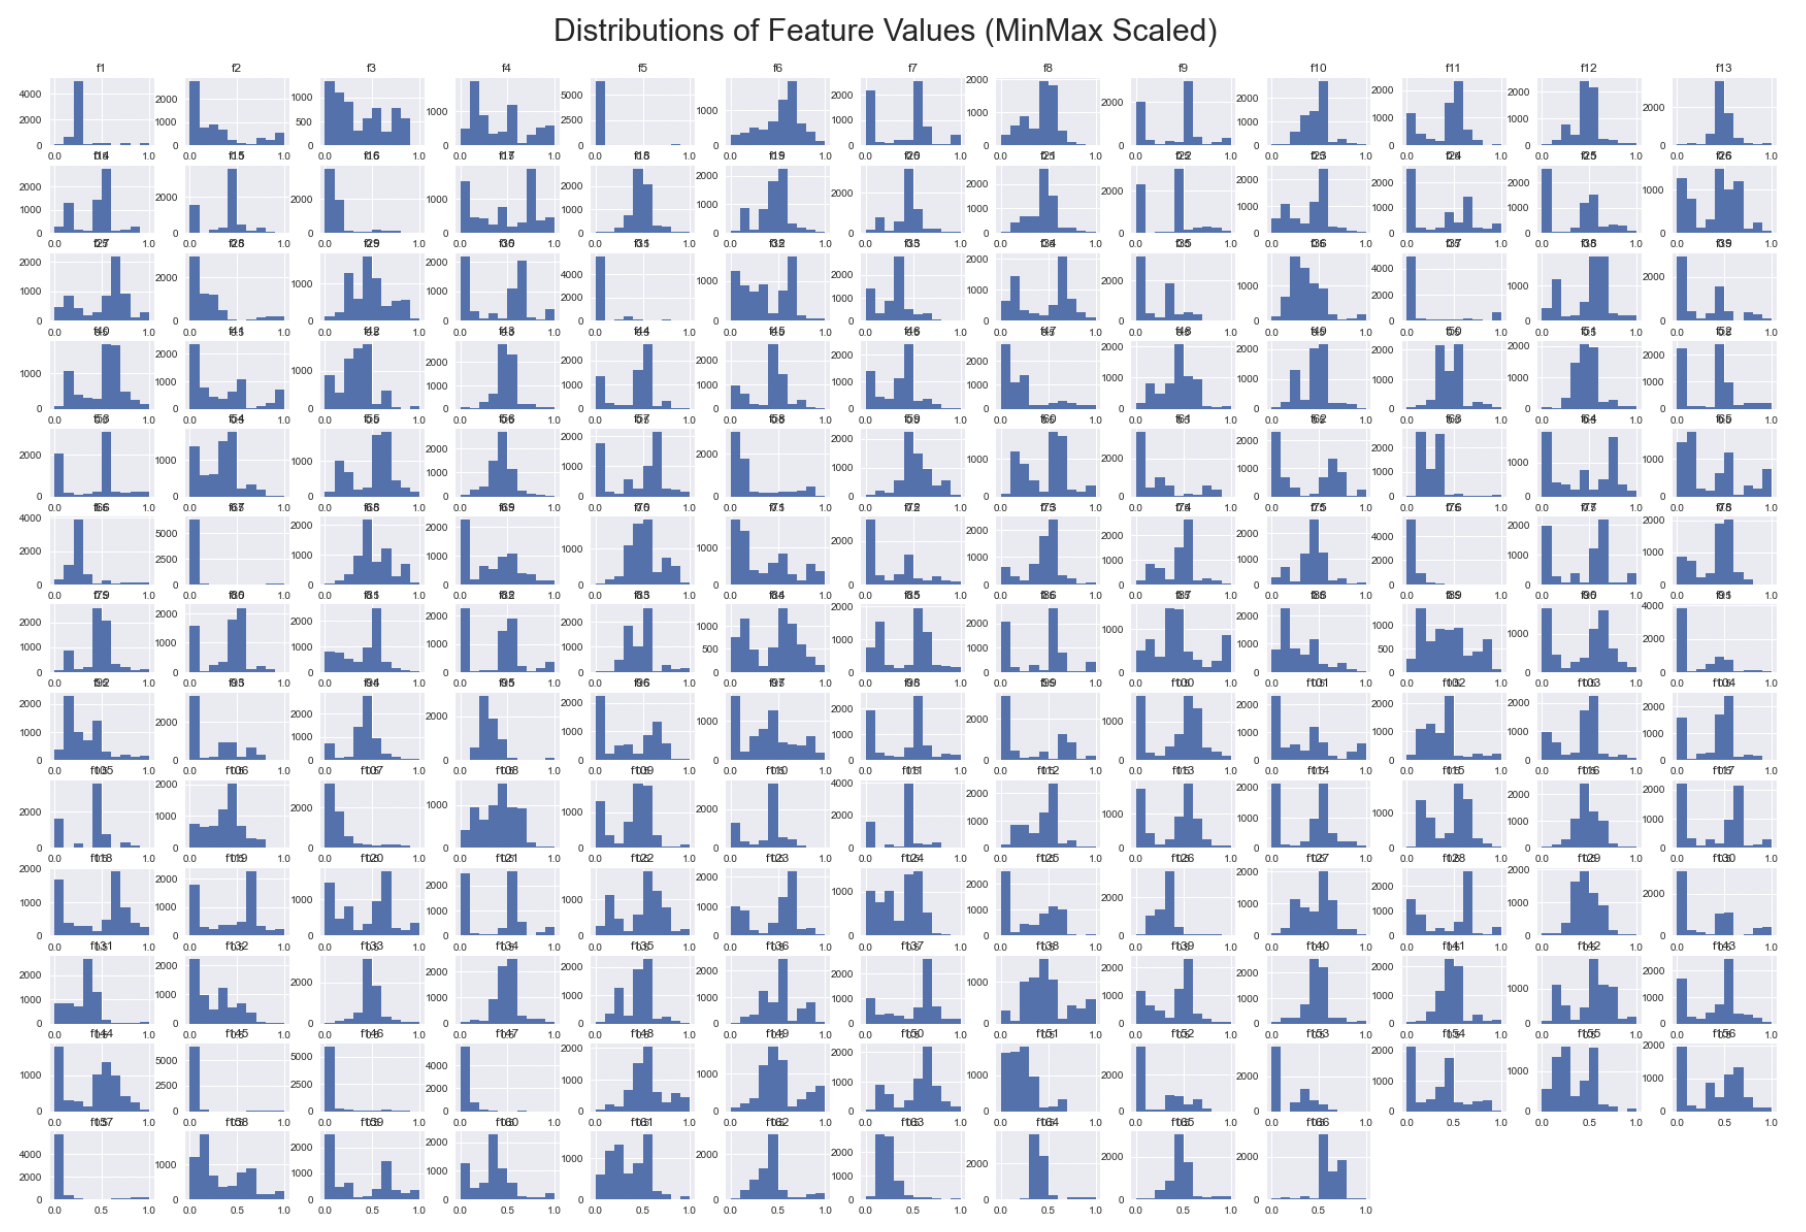
\includegraphics[scale=.47]{feature_distribs.jpg}

As you can see, the features of this data set exhibit a wide variety of distributions, some vaguely normal, others multimodal or even exponential. None appear uniform, so each molecular axis has at least one area along which observations are clustered. Additionally, few if any concentrations of observations occur at the high end of these scaled ranges. This implies that there is a tendency for observations to fall at the lower end of these distances, which are typically negative. The original analysis of this data set says that the 0 points on these axes are arbitrary, so it's hard to glean much meaning from this, but interesting to note nonetheless.

If we look at a histogram compiling all of these scaled observations, we can see these general trends writ large, with the overall mix of distributions combining to make what looks like a normal distribution combined with an exponential distribution. Thus, the molecular distances appear to be drawn from a mixed model.

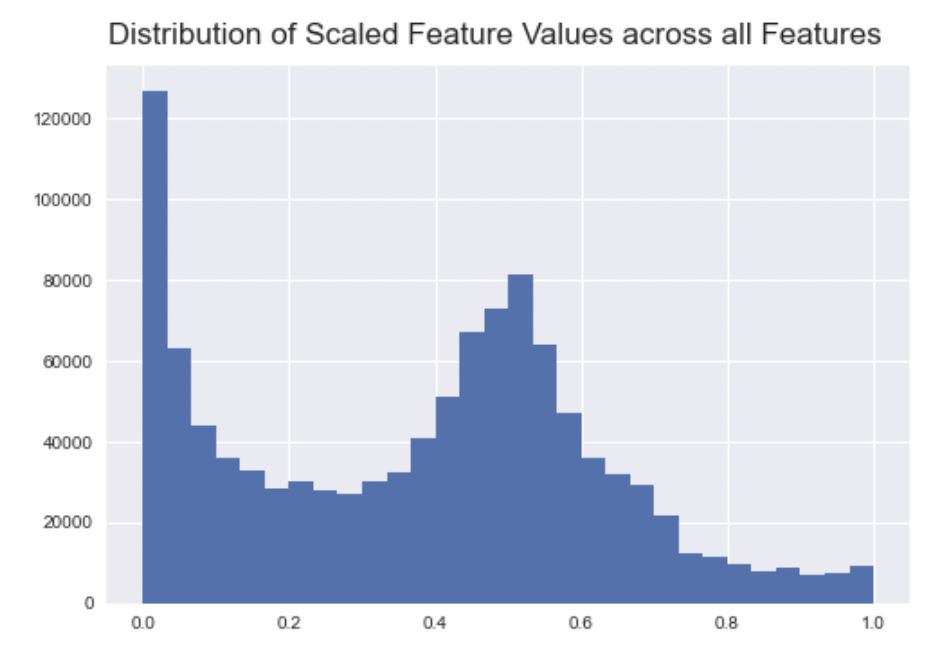
\includegraphics[scale=.8]{all_feature_distrib.jpg}

\textbf{Feature-Feature and Feature-Outcome Correlations}

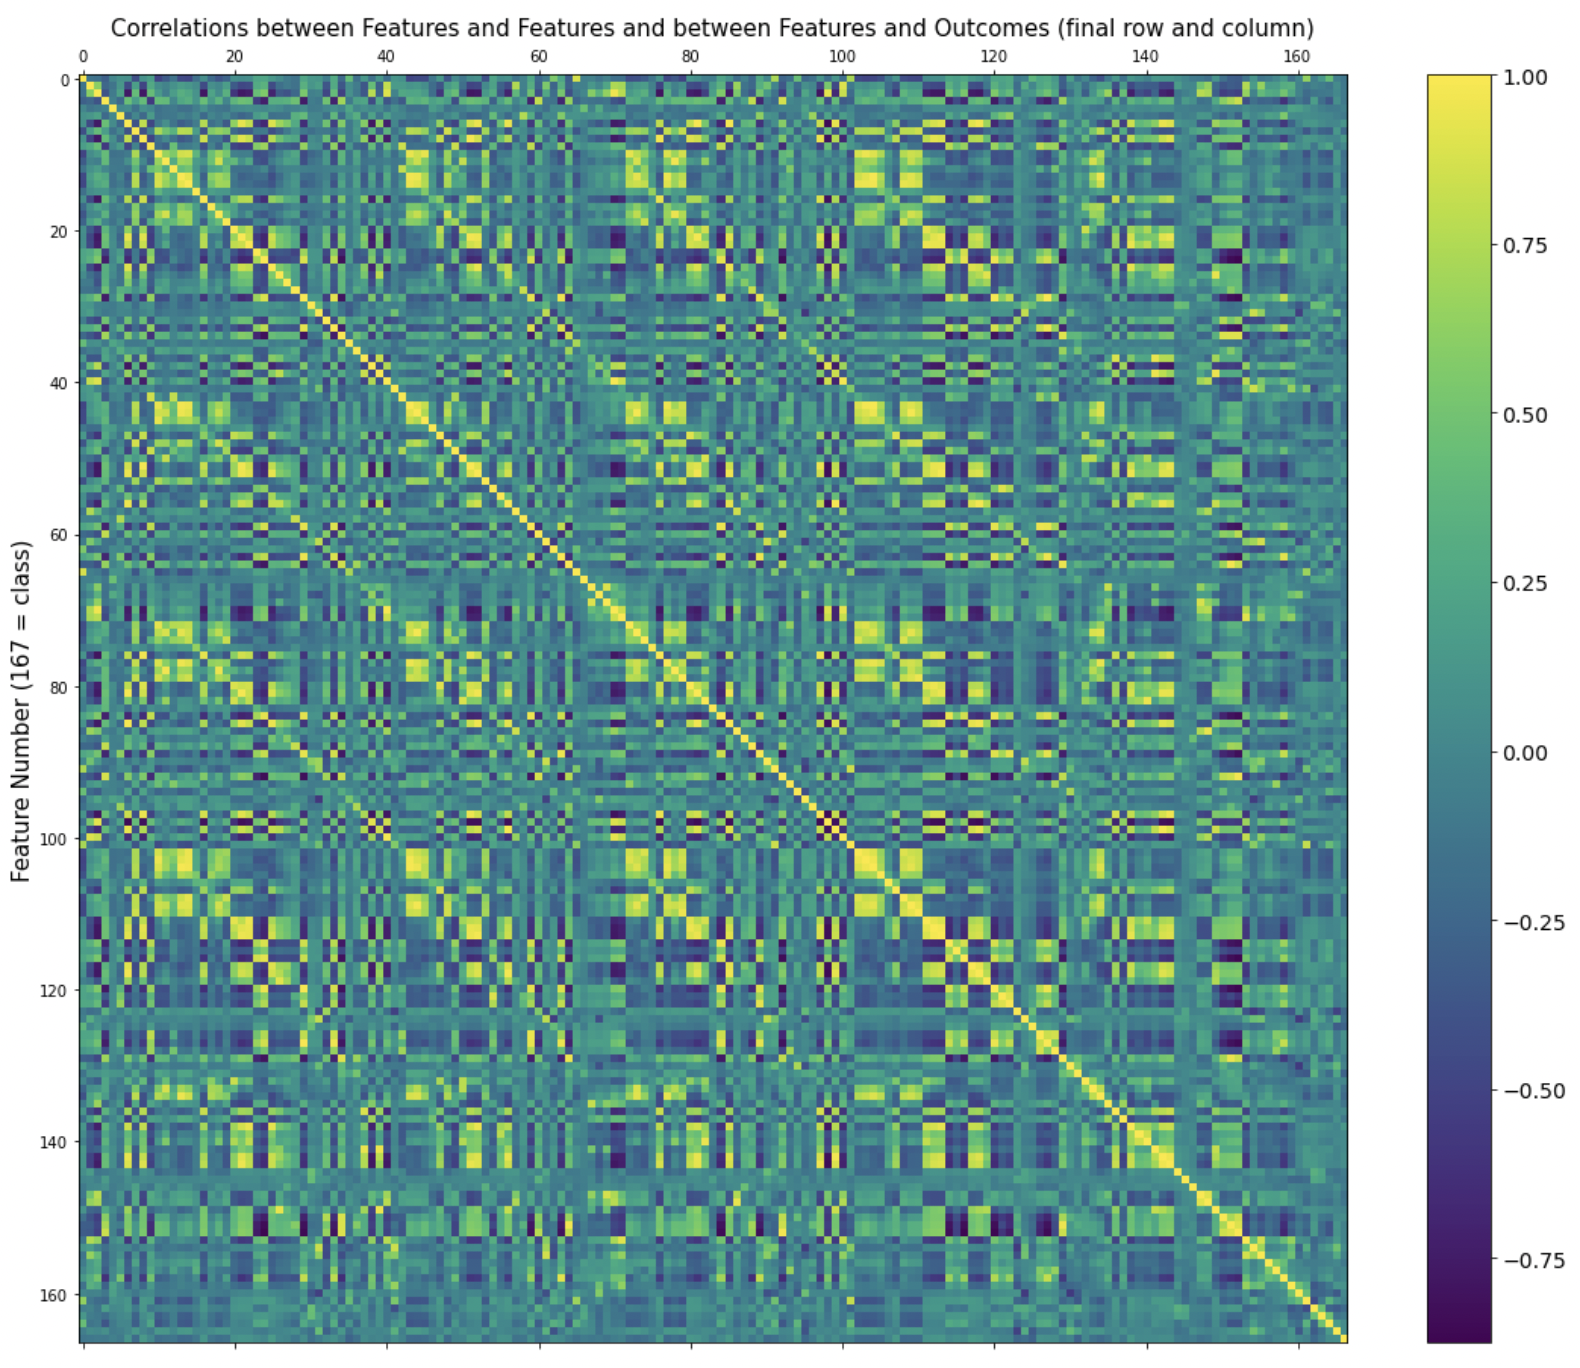
\includegraphics[scale=.6]{correlation_matrix.jpg}

There are some interesting patterns in terms of feature-feature correlations in this data set. As is easily seen in the correlation matrix above, there are a handful of series of successively numbered features that exhibit high positive correlation with other series of successively numbered features. This results in the various diagonal yellow lines around the matrix (not including the main diagonal, of course). We can see that in the feature-feature correlations (all squares except for the last row and column) there are also a large number of highly negative correlations. On the whole, there is quite a range, so it makes sense than when viewed in a histogram, the set of correlations appears to be approximately normally distributed.

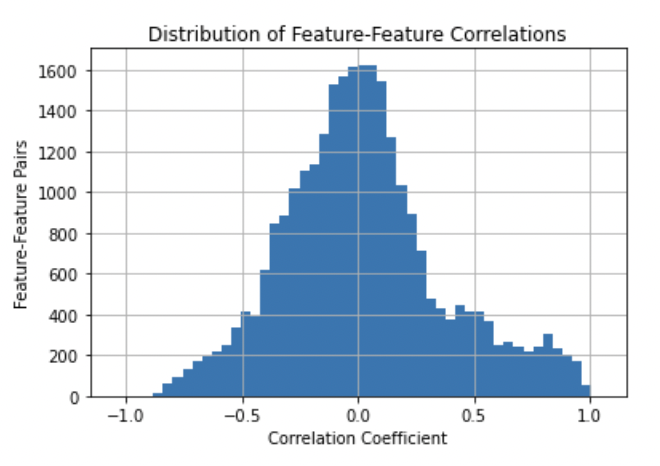
\includegraphics[scale=1.2]{feat_feat_corr_distrib.jpg}

The final row and column of the correlation matrix, which contain feature-outcome correlations, while hard to make out don't appear to have many very high or low values. This visual inspection is confirmed by looking at the distribution of these values. As you can see below, it is much narrower than that of the feature-feature correlations, meaning that no feature is in and of itself highly predictive of outcome. Thus, the whole procedure of training a model using a number of these features makes sense.

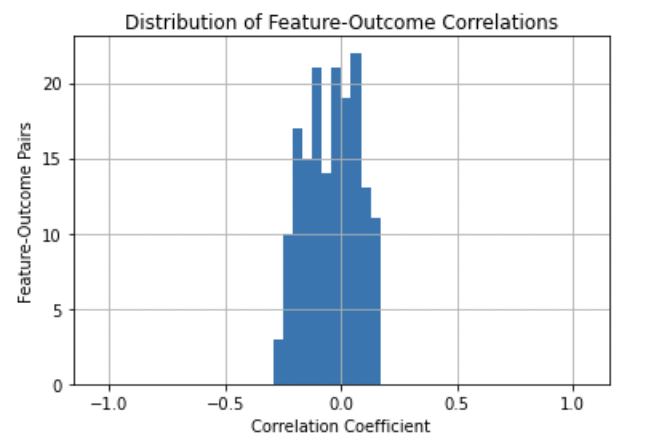
\includegraphics[scale=1.2]{feat_outcome_correlations.jpg}

\textbf{Principal Component Analysis}

As there are many features in our data set and the number of features can have a large effect on the time it takes to train a model, it stands to reason that it might be helpful to reduce this number. By using principal component analysis with increasing numbers of principal components, we were able to see how much variance was retained with each iteration. As you can see from the graph below, we can cut the number of features down to 14 principal components and still retain over 80\% of the original variance. To retain 90\%, we would need 26, and to get 99\%, we would need 74. Even at this high bar, we could reduce our feature set by more than half. This ability to reduce the feature space makes sense in light of the number of features with very high (positive) and very low (negative) correlations.

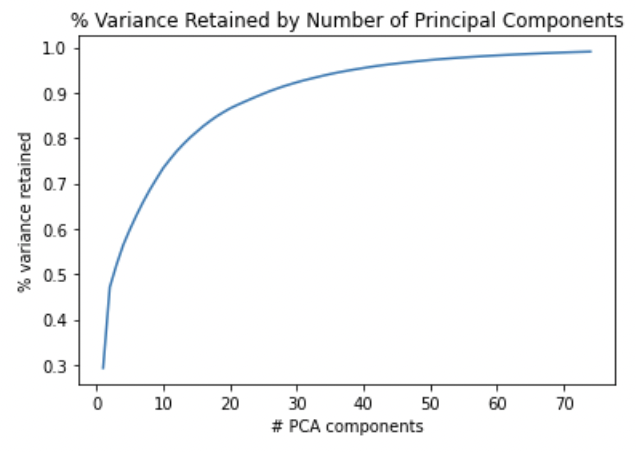
\includegraphics[scale=1.2]{pca_var_retained.jpg}

\textbf{Outcome Distribution}

The outcome distribution is highly imbalanced, with approximately 85\% of the conformations being classified as non-musks. This is even more imbalanced than the molecule outcome distribution, in which approximately 60\% of molecules were judged to be non-musks. This means that non-musk molecules have about 40\% more conformations on average than musk molecules.

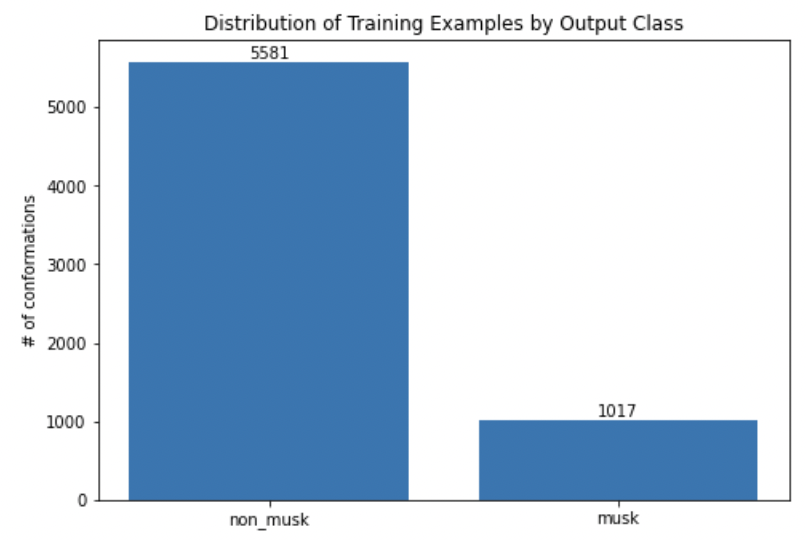
\includegraphics[scale=1]{outcome_distrib.jpg}

For training a logistic classifier, we may need to take this imbalance into account in order to train a model most efficiently. We could account for this aspect of the data either by weighing errors on musk conformations higher than those on non-musks in gradient descent or by using an ensemble model, in which each iteration of the classification model puts a higher weight on the loss associated with observations misclassified by models that came before.

\section{Model and Learning Method Properties}
  

\subsection{Model}

We will be using a logistic regression model with a multivariate Gaussian prior on the weight vector for this data set. The likelihood for this model is the probability of seeing our training data given a certain weight vector. In terms of equations, our prior will look like

\begin{equation}
    w \sim N(\vec{0}, \alpha^{-1}I_{166})
\end{equation}

and our likelihood like

\begin{equation}
    p(x
\end{equation}


With this model, we will compute a MAP estimate of the weight vector after taking the training data into account and use this estimate to predict held-out observations.




\subsection{Learning method (inference)}

\section{Performance Hypotheses}

\end{document}